\documentclass{article}
\usepackage{bm}
\usepackage{amsmath}
\usepackage{graphicx}
\usepackage{mdwlist}
\usepackage[colorlinks=true]{hyperref}
\usepackage{geometry}
\geometry{margin=1in}
\geometry{headheight=2in}
\geometry{top=2in}
\usepackage{palatino}
%\renewcommand{\rmdefault}{palatino}
\usepackage{fancyhdr}
%\pagestyle{fancy}
\rhead{}
\lhead{}
\chead{%
  {\vbox{%
      \vspace{2mm}
      \large
      Introduction to Deep Learning M2177.0043 \hfill
\\
      Seoul National University
      \\[4mm]
      Homework \#(\textbf{HW1})\\
      \textbf{Seo Junwon}
    }
  }
}


\usepackage{paralist}
\usepackage{amsmath}
\usepackage{amssymb}
\usepackage{todonotes}
\usepackage{listings}
\setlength{\marginparwidth}{2.15cm}

\usepackage{tikz}
\usetikzlibrary{positioning,shapes,backgrounds}

\begin{document}
\pagestyle{fancy}

\section*{INSTRUCTIONS}

\begin{itemize*}
\item Anything
  that is received after the deadline will be considered to be late and we do not receive late homeworks. We do however ignore your lowest homework grade. 
\item Answers to every theory questions need to be submitted
  electronically on ETL. Only PDF generated from LaTex is accepted.
\item Make sure you prepare the answers to each question
  separately. This helps us dispatch the problems to different graders.
\item Collaboration on solving the homework is allowed. Discussions
  are encouraged but you should think about the problems on your own. 
\item If you do collaborate with someone or use a book or website, you
  are expected to write up your solution independently.  That is,
  close the book and all of your notes before starting to write up
  your solution. 
\end{itemize*}


%!TEX root = hw1.tex
\section{Q1}

\subsection{}
\begin{center}
    \begin{tabular}{|c | c|}
    \hline
    Junwon & Seo \\
    \hline
    Computer Science \& Engineering & 2017-19428 \\
    \hline
    \end{tabular}
\end{center}

\subsection{}    
\graphicspath{ {images/}}
\begin{center}
    
\includegraphics[width=0.335\textwidth]{junwon.jpg}
\end{center}


%% Q2
\section{Q2}

\subsection{Probability integral transform} 
$F_{Y}(y)$ = $Pr( F_{X}(X) \leq y)$ = $Pr(X \leq F^{-1}_{X}(y))$ = $F_{X}( F^{-1}_{X}(y) )$ = y \\
As $F_{X}$ is a continuous function,\\
$0 \leq F_{X}  \leq 1$.\\
$F_{Y}(y) = y$ for  $0 \leq y \leq 1$.\\
$\therefore$ Y is uniformly distributed in [0,1]\\

\subsection{Inverse transform sampling}
Let $ Y = F^{-1}_{X}(U) $\\
Then the cdf of Y is as follow\\
\[F_{Y}(x) = Pr(F^{-1}_{X}(U) \leq x)\]
\[ \iff F_{Y}(y) = Pr(U \leq F_{X}(x))\]
$Pr(U \leq F_{X}(x))$ = $F_{X}(x)$\\
because, if we constitute $F_{X}(x)$ for simply k\\
$Pr(U \leq k)$ is simply k.\\
Therefore, $F^{-1}_{X}(U)$ has $F_{X}(x)$ for its CDF.

\subsection{Simulation}
\begin{lstlisting}
# (1) analytical PDF of exponential distribution.
import numpy as np
import matplotlib.pyplot as plt
    x = np.linspace(0, 5, 10000)
    lamb = 1
    y = lamb * np.exp(-lamb*x)
    plt.plot(x,y)
\end{lstlisting}
\begin{center}
    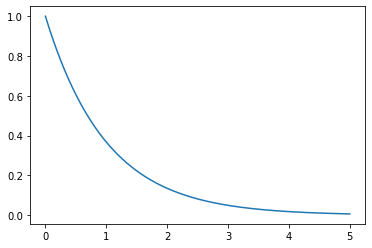
\includegraphics[width=0.6\textwidth]{images/2_3_analy.png}
\end{center}
\begin{lstlisting}
#  (2) normalized histogram of your samples (use 500 bins)
import numpy as np
import matplotlib.pyplot as plt
n = 500
a = np.random.exponential(1., size=1000000)

plt.hist(a, bins=500, density = True)
plt.show()
\end{lstlisting}
\begin{center}
    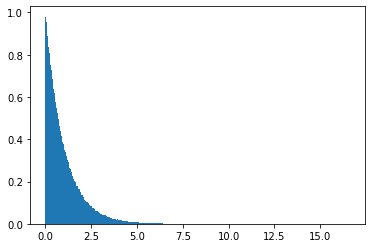
\includegraphics[width=0.6\textwidth]{images/2_3_revised.png}
\end{center}

%% Q3
\section{Q3}
Let's assume I have owned K shares of stock B initially and sold x shares of it.\\
Then the variance of the shares "V" is\\
\[Var( (k-x) X_{B} + X_{A}) \]
\[\iff (k-x)^{2} \sigma^{2}_{B} + \sigma^{2}_{A} + 2 (k-x) \rho \sigma_{B} \sigma_{A} \]
If we differentiate this with respect to $x$,\\
\[ \frac{\partial(V)}{\partial(x)} = -2(k-x)\sigma^{2}_{B} - 2\rho \sigma_{B} \sigma_{A} \]
to Minimize $V$ by $\frac{\partial(V)}{\partial(x)} =0,$ we obtain\\
\[\therefore x = k + \frac{\rho \sigma_{A}}{\sigma_{B}}\]
So if $\rho \geq 0$ we should sell all k shares of B\\
Else if $\rho < 0$ and $x \geq 0$, we should sell $ k + \frac{\rho \sigma_{A}}{\sigma_{B}}$ shares of B

%% Q4
\section{Q4}
$Xv = \lambda v$\\
if $v$ = $(1,1,1,\dots,1)^{T}$,\\
$Xv_{i} = 1+c(p-1), \forall \lambda$\\
$\lambda = 1+c(p-1)$\\
\\
Then the traces of matrix X is p.\\
$ (n-1) * \lambda + (1+c(p-1)) = p $\\
$\lambda = -c + 1$ for $v_{i}$ = $(1,\dots,-p+1,\dots,1)$

%% Q5
\section{Q5}
\subsection{}
$E[Z] = \Vec{0}$\\
$TZ = (TZ_{1}, \dots, TZ_{n})$\\
$\Sigma = Cov(TZ)$ and $\Sigma$ is symmetric.\\ $\Sigma = QDQ^{T} = SS^{T}$. S is generated by eigen decomposition of the covariance matrix, $S = (QD^{1/2})$\\
Let $T = \mu + SZ$\\
$E[TZ] = \mu$ and,
$Cov(TZ) = E[(TZ)(TZ)^{T}] = E[(SZ)(SZ)^{T}] = SE[ZZ^{T}]S^T = \Sigma$\\
$\therefore X = \mu + SZ$ takes Z to $N(\mu,\Sigma)$
\subsection{}
\begin{lstlisting}
# 1) the std normal, 2) your transformed multivariate samples, and 3) multivariate samples obtained from the Numpy code

import numpy as np
import matplotlib.pyplot as plt
import scipy.linalg
sigma = np.array([ [1.0, 0.9], [0.9, 1.0]])
mean = np.zeros(2)
S = scipy.linalg.sqrtm(sigma)

np.random.seed(1337)

z = np.random.normal( size = (2, 10000) ) #std normal

X = np.matmul(S, z) # transformation

y = np.random.multivariate_normal(mean, sigma, 10000) # numpy

plt.subplot(1,3,1)
plt.scatter(z[0], z[1], s=0.5)

plt.subplot(1,3,2)
plt.scatter(X[0], X[1], s=0.5)

plt.subplot(1,3,3)
plt.scatter(y[...,0], y[...,1], s = 0.5)
\end{lstlisting}

\begin{center}
    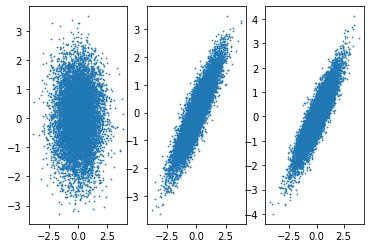
\includegraphics[width=1\textwidth]{images/5.png}
\end{center}
The result of my own quite matches that of the Numpy's, in my humble opinion.

\section{Q6}
$\bigtriangledown f(x^*)^{T}(x-x^*) \geq 0, \forall x \in R^+$\\
Let $x = \Vec{0}$, we obtain \\
\[\bigtriangledown f(x^*)^{T}(x^*) \leq 0 \tag{1} \label{eq:special} \]
As $x^* \in R^+$, if let $x = x^* - x^*_{i}$, s.t $x_{i}^* = (0,\dots,x^*_{i},\dots,0)$, which means $x^*_{i}$ has only $i^th$ component of $x^*_{i}$, otherwise 0.\\
$\forall i, \bigtriangledown f(x^*)$'s ith component $\bigtriangledown f(x^*)_{i}$ satisfies following\\ 
\[f(x^*)_{i}*x^*_{i}   \leq 0 \tag{2} \label{eq:special}\]
which implies $\bigtriangledown f(x^*)  \in R^+$\\
By equation (1), (2), we obtain\\
\[\bigtriangledown f(x^*) = \Vec{0} \]
\[or\]
\[\exists \; i\; s.t \; x^*_{i} = 0\]
as $x \in R^+ $
\end{document}
